% journal.tex
% Template file to use for LLNCS papers prepared in LaTeX
% websites for more information: http://www.springer.com
%http://www.springer.com/lncs

\documentclass{llncs}
\usepackage{setspace}
\usepackage[bahasa]{babel}
\usepackage{graphicx}
%Use this line instead if you want to use running heads (i.e. headers on each page):
%\documentclass[runningheads]{llncs}

\begin{document}
\title{Analisa Unjuk Kerja Format Serialisasi Data JSON dan XML}

%If you're using runningheads you can add an abreviated title for the running head on odd pages using the following
%\titlerunning{abreviated title goes here}
%and an alternative title for the table of contents:
%\toctitle{table of contents title}

%\subtitle{Subtitle Goes Here}

%For a single author
%\author{Author Name}

%For multiple authors:
\author{Muhammad Ghazali\inst{1}}


%If using runnningheads you can abbreviate the author name on even pages:
%\authorrunning{abbreviated author name}
%and you can change the author name in the table of contents
%\tocauthor{enhanced author name}

%For a single institute
%\institute{Institute Name \email{email address}}

% If authors are from different institutes 
\institute{Teknik Informatika, Fakultas Teknik, Universitas Widyatama \\Cikutra No. 204 A Bandung,
Jawa Barat, Indonesia 40124 \email{muhammad.ghazali@widyatama.ac.id}}

\maketitle

\begin{abstract}

\onehalfspacing JSON digunakan untuk merepresentasikan data berbasis teks dalam format yang dapat dikonsumsi dengan mudah oleh aplikasi lain. Penulis memilih format serialisasi data JSON karena JSON lebih mudah ditulis dan dibaca oleh mesin (komputer) dan manusia. Selain itu JSON lebih mudah untuk diproses karena memiliki struktur yang lebih sederhana dibandingkan XML\cite{json-fat-free}\cite{json-vs-xml-debate}\cite{introducing-json}.

\onehalfspacing Penulis membuktikan bahwa data yang diserialisasikan dalam format JSON memiliki ukuran yang lebih kecil dibandingkan XML. Disini penulis hanya membandingkan ukuran data yang dihasilkan setelah dilakukan serialisasi. Hal tersebut dibuktikan dengan membangun purwa-rupa Web API untuk menerapkan JSON pada \textit{resource} yang akan dikonsumsi oleh aplikasi lain. Dengan membangun purwa-rupa Web API ini dibuktikan juga bahwa API yang menserialisasikan data dalam format JSON mampu melayani permintaan \textit{web resource} lebih banyak dibandingkan dengan API yang menserialisasikan data dalam format XML.

Kata kunci: Web API, JSON, Format Serialisasi Data
\end{abstract}

\section{Pendahuluan}

% menjelaskan obyek penelitian
\onehalfspacing Dalam penelitian ini penulis membahas mengenai topik menarik tentang analisa unjuk kerja format serialisasi data JSON dan XML. Hal yang dipelajari adalah untuk membuktikan bahwa data yang diserialisasi dalam format JSON memiliki ukuran data yang lebih kecil jika dibandingkan dengan data yang diserialisasi dalam format XML. Untuk membuktikan hal tersebut penulis mengambil studi kasus implementasi Web API untuk CampusLife \textit{mobile information directory application}.

Web API dibangun dengan tujuan untuk membuka akses secara tidak langsung ke \textit{data store} yang tersimpan di salah satu layanan yang digunakan oleh LLM di AppFog \cite{db-as-a-service}\cite{data-store}. Seluruh data-data \textit{event} yang tersimpan di \textit{data store} akan diolah oleh Web API menjadi data dengan format yang dapat dikonsumsi dengan mudah oleh aplikasi \textit{mobile} CampusLife. Proses pengolahan tersebut dinamakan serialisasi data.

\onehalfspacing Namun, hal yang menjadi fokus di penelitian ini bukanlah tentang implementasi Web API tersebut, melainkan tentang analisa unjuk kerja dari penerapan format serialisasi data ketika data dikirimkan dari Web API ke \textit{client}. Web API hanya akan dibangun sebagai pendukung untuk membantu penulis dalam menganalisa ukuran data yang diformat JSON dan XML ketika dikirimkan ke \textit{client}. Mulai dari bab ini dengan selanjutnya data-data yang yang dikirimkan dari Web API ke \textit{client} akan sering disebut \textit{resource}. 

% Pada bagian ini jelaskan rumusan masalah yang akan diteliti
\onehalfspacing Adapun masalah yang diteliti dalam penelitian ini dapat dirumuskan sebagai berikut:
\begin{enumerate}
  \item Seberapa kecil ukuran \textit{resource} yang diformat dalam JSON jika dibandingkan dengan ukuran \textit{resource} yang diformat dalam XML? 
  \item Bagaimana implikasi terhadap jumlah permintaan  \textit{resource} yang berhasil dikembalikan oleh Web API jika \textit{resource} diformat dalam JSON dan XML?

\onehalfspacing Adapun sistematika penulisan terdiri dari pendahuluan, metodologi, analisis, dan penutup.
\end{enumerate}

\section{Metodologi}
\onehalfspacing Adapun tahapan penelitian yang dilakukan oleh penulis adalah sebagai berikut:
\begin{enumerate}
  \item \textbf{Identifikasi masalah dan perumusan hipotesis}. Pada tahap ini penulis merumuskan masalah yang diteliti.
  \item \textbf{Pengujian format serialiasi JSON dan XML}. Pada tahap ini penulis melakukan pengujian serialisasi dengan membangun purwa-rupa Web API untuk mendukung proses pengujian serialiasi data dalam format JSON dan XML.
  \item \textbf{Analisis unjuk kerja serialisasi}. Pada tahap ini penulis menganalisis unjuk kerja dari format serialisasi JSON dan XML dengan melakukan beberapa skenario pengujian.
  \item \textbf{Merumuskan kesimpulan}. Pada tahap ini penulis membuat kesimpulan hasil analisis dari unjuk kerja format JSON dan XML.
\end{enumerate}

Visualisasi dari tahapan yang dijelaskan di bagian sebelumnya dapat dilihat pada gambar \ref{visualisasi-metodologi}.

\onehalfspacing
\begin{figure}[htp]
\centering
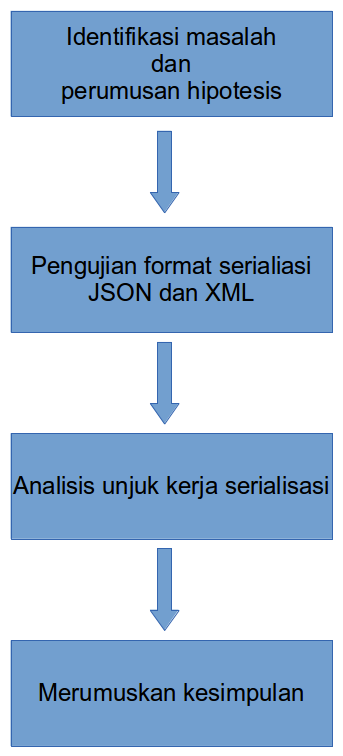
\includegraphics[scale=0.45]{images/visualisasi-metodologi.png}
\caption{Visualisasi Metodologi}
\label{visualisasi-metodologi}
\end{figure}

\section{Analisis}

\subsection{Hasil Pembandingan Antara JSON dan XML}

Penulis melakukan pembandingan antara JSON dan XML dalam hal ukuran data yang dihasilkan dan jumlah respon permintaan yang berhasil dikembalikan ketika Web API diakses oleh \textit{client}. Pembandingan akan dilakukan dengan menggunakan data yang sama dan jumlah detik yang digunakan saat melakukan pembandingan.

Untuk melakukan hal ini penulis menggunakan Apache Benchmark \cite{ab}. Kakas tersebut akan bertugas mengirimkan permintaan Web API \textit{end point} daftar \textit{event}. Berikut adalah skenario pembandingan yang penulis lakukan:

\begin{enumerate}
  \item \textit{Empty Resource}. Melakukan pembandingan jumlah permintaan yang berhasil direspon dengan respon yang dikembalikan berisi \textit{resource} dengan setiap \textit{field} dari \textit{resource} diberi \textit{resource} kosong dengan setiap \textit{field} dari \textit{resource} diberi \textit{string} kosong
  \item \textit{Normal Resource}. Melakukan pembandingan jumlah permintaan yang berhasil direspon dengan respon yang dikembalikan berisi \textit{resource} dengan setiap \textit{field} dari \textit{resource} diberi data yang "normal"
  \item \textit{Just Once}. Melakukan pembandingan ukuran data terhadap hasil respon yang dikembalikan berisi \textit{resource} dengan setiap \textit{field} dari \textit{resource} diberi data yang "normal"
\end{enumerate}

Hasil detail pembandingan dari masing-masing skenario tersebut dapat dilihat di bagian selanjutnya.

\subsection{Hasil Pembandingan Skenario Empty Resource}

\onehalfspacing \textit{Empty Resource}. Melakukan pembandingan jumlah permintaan yang berhasil direspon dengan respon yang dikembalikan berisi "\textit{resource} kosong" dengan setiap \textit{field} dari \textit{resource} diberi \textit{string} kosong. Representasi dalam bentuk grafik dari hasil pembandingan tersebut dapat dilihat pada gambar \ref{benchmark-empty-resource}.

\begin{figure}[htp]
\centering
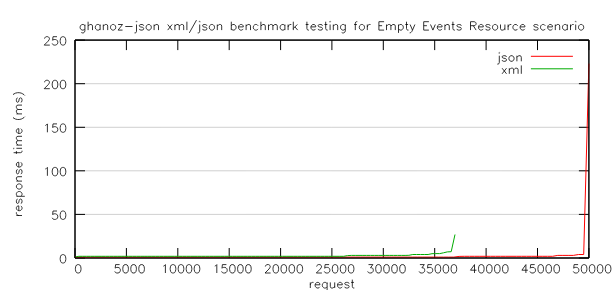
\includegraphics[scale=0.65]{images/benchmark-empty-resource.png}
\caption{Perbandingan Jumlah Permintaan yang berhasil direspon untuk skenario Empty Resource}
\label{benchmark-empty-resource}
\end{figure}

Bisa dilihat melalui grafik di atas, bahwa dalam 73,853 detik, Web API mampu mengembalikan respon dari 50000 permintaan dalam format JSON. Sedangkan dalam 90 detik, Web API hanya mampu mengembalikan respon dari 36973 permintaan dalam format XML.

\subsection{Hasil Pembandingan Skenario Normal Resource}

\onehalfspacing \textit{Normal Resource}. Melakukan pembandingan jumlah permintaan yang berhasil direspon dengan respon yang dikembalikan berisi \textit{resource} dengan setiap \textit{field} dari \textit{resource} diberi data yang "normal". Representasi dalam bentuk grafik dari hasil pembandingan tersebut dapat dilihat pada gambar \ref{benchmark-normal-resource}.

\begin{figure}[htp]
\centering
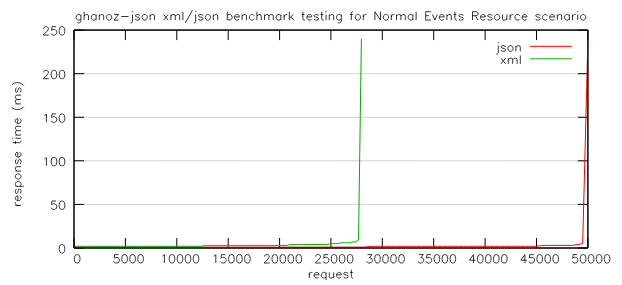
\includegraphics[scale=0.65]{images/benchmark-normal-resource.png}
\caption{Perbandingan Jumlah Permintaan yang berhasil direspon untuk skenario Normal Resource}
\label{benchmark-normal-resource}
\end{figure}

Bisa dilihat melalui grafik di atas, bahwa dalam 87.414 detik, Web API mampu mengembalikan respon dari 50000 permintaan dalam format JSON. Sedangkan dalam 90 detik, Web API hanya mampu mengembalikan respon dari 27966 permintaan dalam format XML.

\subsection{Hasil Pembandingan Skenario Just Once}

\onehalfspacing \textit{Just Once}. Melakukan pembandingan ukuran data terhadap hasil respon yang dikembalikan berisi \textit{resource} dengan setiap \textit{field} dari \textit{resource} diberi data yang "normal". Berikut detail hasil pembandingannya:

\begin{enumerate}
  \item Ukuran data \textit{resource} dalam format JSON dengan besar 4377 \textit{bytes} berhasil direspon oleh Web API dalam waktu 0,0004 detik
  \item Ukuran data \textit{resource} dalam format XML dengan besar 6635 \textit{bytes} berhasil direspon oleh Web API dalam waktu 0,0005 detik
\end{enumerate}

\section{Penutup}

\subsection{Kesimpulan}

Selama menjalani masa penelitian penulis mendapatkan beberapa kesimpulan dari hasil penerapan JSON sebagai format serialisasi data:

\begin{enumerate}
  \item Berdasarkan hasil pengujian yang sudah dilakukan, terbukti bahwa data yang diserialisasi dalam format JSON memiliki ukuran data yang lebih kecil jika dibandingkan dengan data yang diserialisasi dalam format XML.
  \item Implikasi dari penerapan JSON pada \textit{resource} adalah jumlah permintaan yang berhasil dikembalikan jauh lebih banyak dibandingkan ketika Web API mengembalikan \textit{resource} dalam format XML.
\end{enumerate}

\subsection{Saran}

Untuk mengembangkan hasil penelitian ini, penulis menyarankan beberapa topik pengembangan berikut:

\begin{enumerate}
  \item Membandingkan JSON secara eksplisit dengan beberapa format serialisasi yang lain dalam hal keunggulan dan kelemahan
  \item Melakukan pengujian Web API dengan mengaksesnya melalui aplikasi
  \item Meneliti isu-isu keamanan ketika menerapkan JSON
  \item Menganalisa trend penggunaan format serilisasi data tertentu  
  \textit{mobile}
\end{enumerate}

Demikian saran-saran yang dapat penulis sampaikan, penulis berharap laporan ini dapat bermanfaat bagi semua pihak yang membaca.

%The bibliography, done here without a bib file
%This is the old BibTeX style for use with llncs.cls
\bibliographystyle{splncs}

%Alternative bibliography styles:
%the following does the same as above except with alphabetic sorting
%\bibliographystyle{splncs_srt}
%the following is the current LNCS BibTex with alphabetic sorting
%\bibliographystyle{splncs03}
%If you want to use a different BibTex style include [oribibl] in the document class line

\begin{thebibliography}{1}
%add each reference in here like this:

\bibitem[1]{json-vs-xml-debate}
Marinescu, Floyd dan Tilkov, Stefan. "Debate: JSON vs. XML as a data interchange format." \emph{Infoq}. Web. 20 Januari 2013. http://www.infoq.com/news/2006/12/json-vs-xml-debate

\bibitem[2]{json-fat-free}
"JSON: The Fat-Free Alternative to XML." \emph{JSON Official Website}. Web. 20 Januari 2013. http://www.json.org/xml.html

\bibitem[3]{introducing-json}
"Introducing JSON" \emph{JSON Official Website}. Web. 20 Januari 2013. http://www.json.org/

\bibitem[4]{db-as-a-service}
"Database as a service" \emph{Wikipedia}. Web. 20 Januari 2013. http://en.wikipedia.org/wiki/Cloud\_database

\bibitem[5]{data-store}
"Data Store" \emph{Wikipedia}. Web. 20 Januari 2013. http://en.wikipedia.org/wiki/Data\_store

\bibitem[6]{ab}
"Apache HTTP server benchmarking tool" \emph{Apache HTTP server benchmarking tool}. Web. 20 Januari 2013. http://httpd.apache.org/docs/2.4/programs/ab.html

\end{thebibliography}

\end{document}

